\section{Je reconnais les trois états physiques (3 poinst)}

Voici des récipients contenant des substances à l'état solide, à l'état liquide et à l'état gazeux.

\begin{questions}
	\question[3] En justifiant la réponse, indiquer l'état représenté dans chaque cas.
	%\begin{multicols}{2}
		
		\begin{center}
			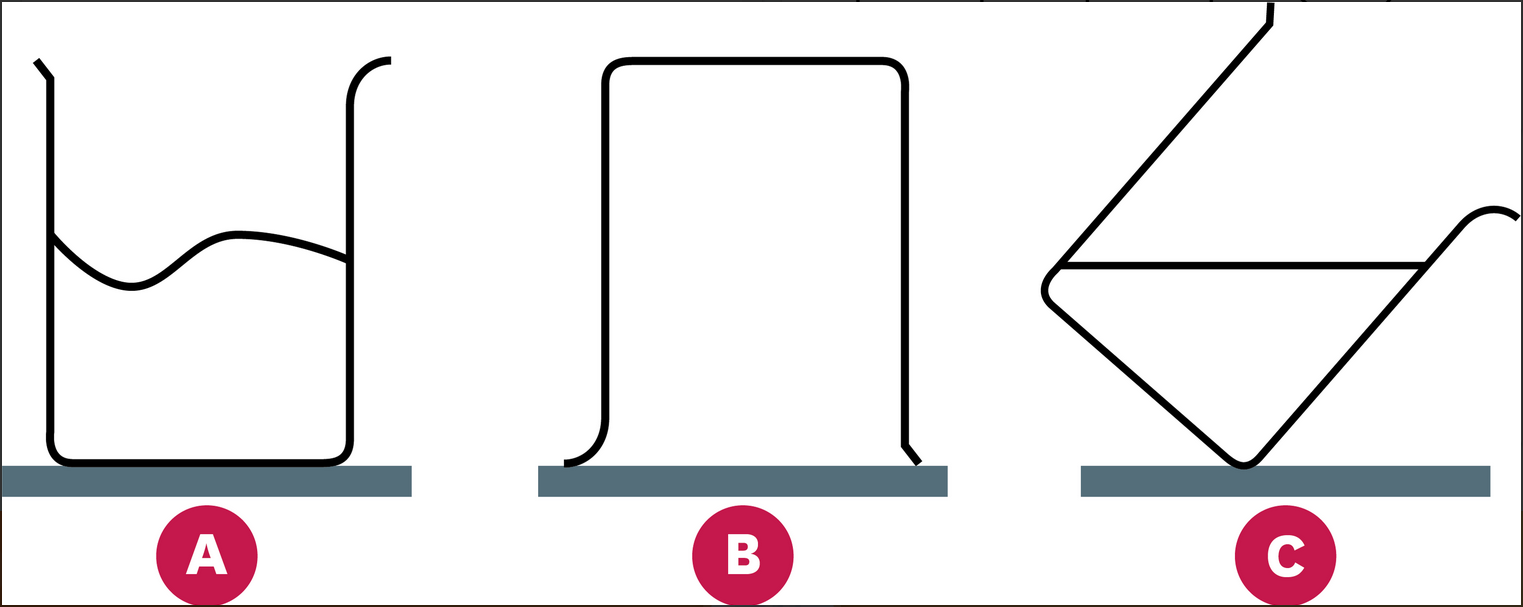
\includegraphics[scale=0.4]{img/reco1}
		\end{center}
	
	\begin{solution}
		\begin{itemize}
			\item Le contenu du bécher A n'a pas de surface libre plane donc c'est un solide.
			
			\item Le contenu du bécher B occupe tout l'espace disponible c'est un gaz.
			
			\item Le contenu du bécher C a une surface libre plane et horizontale donc c'est un liquide.
		\end{itemize}
	\end{solution}


		%\begin{center}
		%	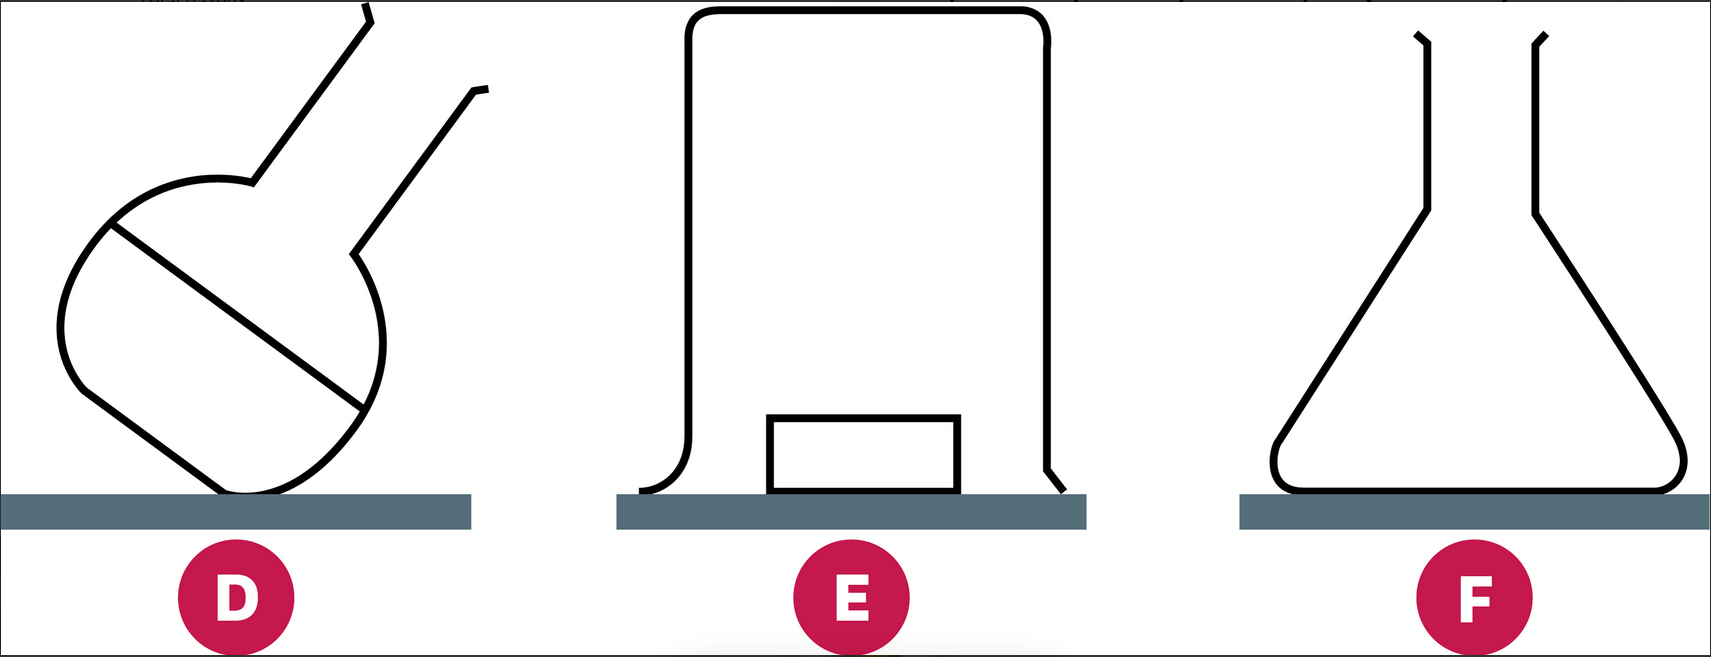
\includegraphics[scale=0.22]{img/reco2}
		%\end{center}
%		\begin{solution}
%			\begin{itemize}
%				\item Le contenu du bécher D n'a pas de surface libre horizontale donc c'est un solide.
%				
%				\item Le contenu du bécher E a une forme propre, c'est un solide.
%				
%				\item Le contenu du bécher F occupe tout l'espace disponible c'est un gaz.
%			\end{itemize}
%		\end{solution}

	%\end{multicols}
\end{questions}